\chapter{Diagnostic de l'image}
\label{chap:chapter_4}
\chapterintro
Comme évoqué durant le préambule, cette partie s'intéresse au premier niveau de diagnostic, c'est à dire celui de l'image sur données \gls{rcm}. La séparation sur problématique binaire, malin et non malin, sera ainsi évaluée mais également sur trois classes avec d'une part les tissus sains, bénin et malin.\par

Ainsi, plusieurs aspects se distinguerons dans ce chapitre dont l'extraction de caractéristiques pertinentes par méthodes manuelles et auto déterminée et l'utilisation de méthodes de classification éprouvées. Nous nous intéresserons également à l'influence de divers paramètres liés à la normalisation des caractéristiques, à la réduction de l'information dans le cadre des méthodes sur base d'apprentissage par transfert et enfin sur l'influence des données sur les résultats obtenus.\par	

\newpage

\section{Méthodologie}
La classification de la peau par méthode d'apprentissage est un problème très largement développée dans la littérature, notamment pour le mélanome. Néanmoins, dans le cadre de la détection du \gls{lm}/\gls{lmm} sur base d'images \gls{rcm},
cette problématique n'a été abordé que par quelques articles~\cite{Halimi2017a, Halimi2017b, Wiltgen2008, Koller2011}. Nous nous intéresserons à la détection de cette pathologie au sein de la base d'image mise à disposition, et nous étudierons cette problématique selon divers angles d'approche: 
\begin{inlinerate}
    \item la séparation entre les tissus malin et le reste des tissus (problématique à 2 classes),
    \item la séparation entre les tissus pathologiques  et les tissus qualifiés de sains (problématique à 2 classes),
    \item et enfin la séparation des tissus malins, bénins et sains (problématique à 3 classes).
\end{inlinerate}\par

Afin de traiter ces problématiques, nous aborderons ces cas à l'aide de mécaniques liées à l'apprentissage supervisé, que nous déroulerons lors de prochains paragraphes. En effet, ces mécaniques ont largement été employé et démontrée fonctionnelles dans des problèmes similaires de classification d'images médicales. Dans un premier temps, nous décrirons le processus par apprentissage automatique ( voir \Cref{fig:scheme_macro_pipeline} - en haut): nous décrirons bloc par bloc les traitements proposés de l'extraction de caractéristique à l'étape de classification. Dans un second temps, nous décririons le processus d'apprentissage profond ( voir \Cref{fig:scheme_macro_pipeline} - en bas): nous traiterons de l'augmentation des données et proposerons une méthodologie d'entraînement. Enfin, nous terminerons par une descriptions des résultats obtenus, tenterons d'expliquer ces derniers, et déterminerons les choix les plus cohérents pour la suite.\par

\begin{figure}[H]
\centering
    \begin{subfigure}{\textwidth}
      \centering
      Processus par apprentissage automatique
      \includegraphics[width=\linewidth]{contents/chapter_4/resources/scheme_macro_pipeline_machine.pdf}
    \end{subfigure}
    \begin{subfigure}{.45\textwidth}
      \centering
      Processus par apprentissage profond
      \includegraphics[width=\linewidth]{contents/chapter_4/resources/scheme_macro_pipeline_cnn.pdf}
    \end{subfigure}
    \caption{Représentation macroscopique du processus de diagnostic image suivi. En haut, le processus macroscopique liée au processus d'apprentissage automatique; En bas, le processus macroscopique liée à l'apprentissage profond.}
    \label{fig:scheme_macro_pipeline}
\end{figure}\par

\newpage

\section{Processus d'apprentissage automatique}
Cette section se destine à présenter l'ensemble des étapes consacrée à la classification des images de \gls{rcm} selon un processus d'apprentissage automatique. Celui-ci se décompose en quatre étapes majeures:
\begin{inlinerate}
    \item l'extraction de caractéristiques,
    \item le balancement des données,
    \item le post traitement,
    \item et la classification
\end{inlinerate}.
Le pré traitement des images n'est pas considéré car jugé peu utile sur ces dernières. Ce processus sera décrit point par point lors des prochaines sous-parties.

\subsection{Extraction de caractéristiques}
L'étape d'extraction de caractéristiques consiste en l'obtention de valeurs dérivées à partir des données brute dans le but de quantifier un phénomène jugée pertinent pour la suite du traitement (généralement de la classification). Les éléments présentés en \Cref{chap:preamble_microscopy} portent à montrer l'importance des motifs de tissus, très variables selon:
\begin{itemize}
    \item la profondeur d'acquisition : l'épiderme, \gls{dej} et le derme sont très différents du point des tissus,
    \item la pathologie à identifier : les différentes lésions en notre possession sont assez différentes selon leur états bénin ou malin.
\end{itemize}\par

Les nombreux échanges menés auprès des spécialistes en dermatologie ont également abouti sur une importance des aspects des textures au sein de leur processus cognitifs de décision vis à vis des pathologies de \gls{lm}/\gls{lmm}.\par

Nous traiterons des techniques d'extraction de caractéristiques appliquée à notre thématique, que nous aborderons selon deux axes:
\begin{inlinerate}
    \item d'une part les techniques d'extraction de caractéristiques manuelles,
    \item d'autre part les techniques d'extraction de caractéristiques non manuelles
\end{inlinerate}. Ces termes ont été utilisés suite à l'apparition de réseaux de convolution profonds, afin de catégoriser ces deux types d'approches~\cite{Nanni2017}.\par

L'extraction de caractéristiques est une problématique qui a été traitées sous deux aspects distincts: l'une par utilisation du domaine spatial et l'autre par utilisation du domaine fréquentiel. Ainsi, ces prochaines lignes traiterons la problématique dans cet ordre respectif.\par

\subsubsection{Extraction de caractéristiques manuelles spatiales}
L'extraction sur base d'information du domaine spatial est un champs de travail assez développé présentant comme avantage d'être intuitif mais pouvant être affecté par le bruit et distorsions. Ces opérations spatiales peuvent être décrites à deux niveaux: les descripteurs de premier ordre ne prenant en compte que les valeurs d'intensités initiales et est indifférent aux information de voisinage; et les descripteurs de second ordre et plus, prenant en compte la relation d'une valeur locale et de son voisinage~\cite{Kamila2015}.\par

Les descripteurs de premier ordre s'appliquent ainsi aux valeurs d'intensité ou à la distribution de celle-ci, sans traitement préalable. La \Cref{tab:first_order_descriptors} recense la plupart des ces mesures. Néanmoins, ces mesures tendent à ressortir des phénomènes globaux de l'image mais ne suffisent pas à elles seules à analyser  des motifs présent, mais peuvent constituer un bon complément ~\cite{Tomita1990, Srinivasan2008}.\par

\begin{table}[H]
    \centering
    \begin{tabular}{ll}
        \hline
        \textbf{Mesure}             & \textbf{Formule}                                                  \\ \hline
        Moyenne                     & $\overline{x} = {1 \over n} \sum_{i=1}^n{x_i}$                    \\     
        Minimum                     & $\min{(x,y)}=\frac{x+y-|x-y|}2$                                   \\    
        Maximum                     & $\max{(x,y)}=\frac{x+y+|x-y|}2$                                   \\  
        Médiane                     & \\      
        Variance                    & \\ 
        Déviation moyenne           & \\
        Erreur quadratique moyenne  & \\ 
        Déviation standard          & \\ 
        Difference                  & \\
        Energy                      & \\
        Entropy                     & \\
        Kurtosis                    & \\
        Skewness                    & \\      
        Uniformity                  & \\  
    \end{tabular}
    \caption{Liste de différentes mesures obtenues à partir du premier ordre.}
    \label{tab:first_order_descriptors}
\end{table}\par


Les descripteurs de second ordre, ou plus, utilisent l'information locale et en déduisent une relation à leur voisinage par l'utilisation généralement d'une transformation intermédiaire. Parmi ces transformation, les plus courantes sont: 
\begin{inlinerate}
    \item \gls{glcm},
    \item \gls{glrlm},
    \item et \gls{glszm}.
\end{inlinerate} 
L'extraction sur la base d'information du second ordre à notamment été traitée en 1973 pour de la reconnaissance d'image aérienne et satellites, par Robert Haralick~\cite{Haralick1973}. Ce travail est une extension des \gls{glcm}, dont le principe consiste en un recensement des combinaisons d'intensité présentent dans une image. Cette extraction nécessite une direction dans laquelle les combinaisons seront recherchées, en 2D ces directions sont aux nombre de quatre:
\begin{inlinerate}
    \item horizontale,
    \item verticale,
    \item et les deux diagonales opposées
\end{inlinerate}. Le principe de fonctionnement des \gls{glcm} est schématisé en \Cref{fig:scheme_principle_GLCM} pour une extraction selon la direction horizontale. Le travail~\cite{Haralick1973} à ainsi démontré la pertinence des \gls{glcm} dans la différenciation d'images texturés, en calculant quatorze critères statistiques selon les quatre directions évoqué précédemment. La \Cref{tab:haralick_descriptors} met à disposition les diverses mesures utilisées et formules associées. Afin de réaliser ces diverses extraction de manière optimum, nous nous référé à la bibliothèque logicielle "Mahotas"~\cite{coelho2012} proposant ces diverses mesures de manière optimisée.\par
 
\begin{figure}[H]
    \centering
    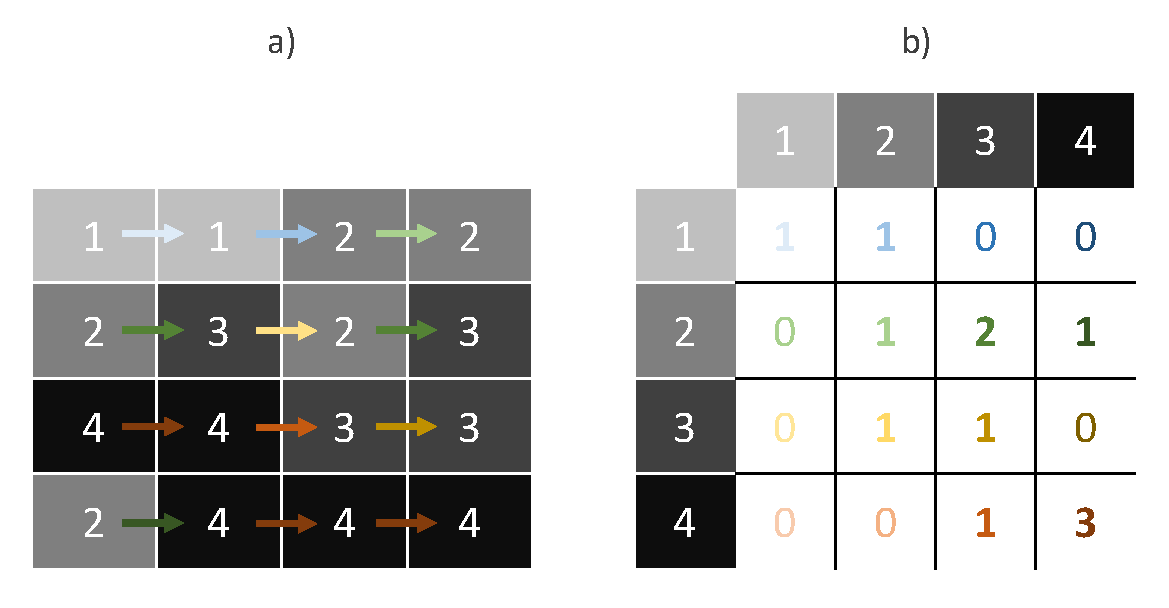
\includegraphics[width=0.8\linewidth]{contents/chapter_4/resources/scheme_principle_GLCM.pdf}
    \caption{Représentation de la création d'une matrice sur base de \gls{glcm} selon la direction horizontale.}
    \label{fig:scheme_principle_GLCM}
\end{figure}\par

L'un des travaux menée par une étude sur les lésions mélanocytaire en \gls{rcm} vont dans le sens de ces deux formes d'information~\cite{Wiltgen2008}. En effet, l'étude met en avant l'importance des douze première caractéristiques énoncés par Haralick et adjoint cinq mesure de premier ordre comme complément d'information dont :
\begin{inlinerate}
    \item la moyenne,
    \item l'erreur quadratique moyenne,
    \item l'asymétrie de la répartition de l'histogramme,
    \item le kurtosis (mesure d'aplatissement de la distribution),
    \item et l'entropie.
\end{inlinerate}
De plus, afin de rendre les caractéristiques d'Haralick plus robuste aux rotations et par la même de réduire la quantité d'information, les auteurs préconise l'utilisation d'une moyenne sur les quatre directions, dont résulte un unique vecteur de taille 1$\times$12~\cite{Wiltgen2008}.\par

\begin{table}[H]
    \centering
    \begin{tabular}{ll}
        \hline
        \textbf{Nom}                & \textbf{Formule}                                                                              \\ \hline
        Angular Second Moment       & $ \sum_i\sum_jp(i,j)^2$                                                                       \\
        Contrast                    & $\sum_{k=0}^{N_g-1} k^2 p_{x-y}(k)$                                                           \\
        Correlation                 & $\frac{\Large{\sum_{i=1}^{N_g}\sum_{j=1}^{N_g}} (ij)p(i,j) - \mu_x\mu_y}{\sigma_x\sigma_y}$   \\
        Sum of Squares: Variance    & $\sum_{i=1}^{N_g}\sum_{j=1}^{N_g} (i - \mu)^2 p(i,j)$                                         \\
        Inverse Difference Moment   & $\sum_{i=1}^{N_g}\sum_{j=1}^{N_g} \frac{1}{1 + (i - j)^2} p(i,j)$                             \\     
        Sum Average                 & $\sum_{i=2}^{2N_g} i p_{x+y}(i)$                                                              \\    
        Sum Variance                & $\sum_{i=2}^{2N_g} (i - f_8)^2 p_{x+y}(i)$                                                    \\    
        Sum Entropy                 & $\sum_{i=2}^{2N_g} (i - f_8)^2 p_{x+y}(i)$                                                    \\    
        Entropy                     & $-\sum_{i=1}^{N_g}\sum_{j=1}^{N_g} p(i,j) \log(p(i,j))$                                       \\    
        Difference Variance         & ${\rm variance \ of ~} p_{x-y}$                                                               \\    
        Difference Entropy          & $-\sum_{i=0}^{N_g-1} p_{x-y}(i) \log(p_{x-y}(i))$                                             \\
        Measure of Correlation 1    & $\frac{f_9 - HXY1}{\max(HX,HY)}$                                                              \\  
        Measure of Correlation 2    & $[1 - \exp(-2(HXY2 - f_9))]^{1/2}$                                                            \\ 
        Maximal Correlation Coefficient    & $({\rm second \ largest \ eigenvalue \ of ~} Q)^{1/2}$ $\sum_k \frac{p(i,k)p(j,k)}{p_x(i)p_y(k)}$ \\ 
    \end{tabular}
    \caption{Liste des des différentes mesures proposé par Robert Haralick applicable aux \gls{glcm}.}
    \label{tab:haralick_descriptors}
\end{table}\par
 
Les expériences menées sur base de descripteurs manuels spatiaux se décomposerons en plusieurs temps. Tout d'abord, nous procéderons à une étude de l'importance séparée des mesures sur l'information de premier ordre et sur les mesures proposée par Haralick sur l'information de second ordre. Nous profiterons de l'expérience pour mesurer l'impact de la moyenne dans cette tâche. Dans un second temps, nous réemploierons la démarche de combinaison conjointe de ces mesures menée par l'un des articles~\cite{Wiltgen2008}. Par ailleurs, la \Cref{tab:number_features_spatial} synthétise l'ensemble des méthodes d'extraction ainsi que le nombre associé de caractéristiques extraites.\par
\begin{table}[h]
\centering
    \begin{tabular*}{0.6\linewidth}{l@{\extracolsep{\fill}}l}
        \hline
        \textbf{Méthode}                            & \textbf{Nombre}   \\ \hline
        Mesures premier ordre                       & 14                \\ \hline
        Haralick~\cite{Haralick1973} - 4 directions & 56                \\ \hline
        Haralick~\cite{Haralick1973} - Moyenne      & 14                \\ \hline
        Wiltgen~\cite{Wiltgen2008} - Spatial        & 17 (12+5)         \\ \hline
    \end{tabular*}
    \caption{Nombre de caractéristiques extraites par méthodes manuelles spatiale.}
    \label{tab:number_features_spatial}
\end{table}

\subsubsection{Extraction de caractéristiques manuelles fréquentielles}
L'extraction sur base d'information du domaine fréquentiel est également un champs de travail assez développé, notamment pour sa robustesse face au perturbation telle que le bruit, ainsi que la vitesse d'exécution de certaines opérations telle que le filtrage. En revanche, l'information extraites est moins évocatrice et nécessite une information spatiale initiale suffisante pour être juste~\cite{Kamila2015}. Plusieurs courants majeurs de représentation sont utilisés: 
\begin{itemize}
    \item la Transformée de Fourier~\cite{Ursani2007, Smach2008a},
    \item la Transformée en cosinus discrète~\cite{Sorwar2001},
    \item la Transformée en ondelettes~\cite{Arivazhagan2003,Hong2010},
    \item et la Transformée de Gabor~\cite{Ursani2007}.
\end{itemize}
Notre travail se consacrera à deux de ces approches, la transformée de Fourier et à la transformée en ondelettes, toutes deux traités sur une problématique similaire~\cite{Wiltgen2008,Halimi2017a,Halimi2017b}. Également, ces deux méthodes sont deux représentants majeures des deux grandes familles de représentation en fréquence.\par

La transformée de Fourier se résume à la décomposition d'une donnée en une somme de fréquences. Dans le cas d'une image, cette transformation donne lieu à une représentation, dans lesquelles: les basses fréquences, au centre, représentent une forme d'homogénéité au sein d'une image; tandis que les hautes fréquences, en extérieur, sont associées à de fortes transitions. Cet espace est donc approprié à la caractérisation d'image texturées, et à suscité un intérêt au milieu des années 1980~\cite{Persoon1986}. En revanche, bien que cette représentation permette de décrire parfaitement la composition fréquentielle de l'image, elle ne peut en localiser la provenance exacte~\cite{Wiltgen2008}. Différentes  mesures ont été proposés dans cet espaces afin de caractériser des textures:
\begin{itemize}
    \item l'extraction d'information à partir \textbf{de cercles concentriques} réguliers~\cite{Smach2008a, Wiltgen2008} afin d'isoler l'information propre à chaque intervalle de fréquences (\Cref{fig:scheme_fourier_features} - a),
    \item l'extraction d'information à partir \textbf{de directions} en partance du centre vers l'extérieur de la transformée à angles constants ~\cite{Wiltgen2008} (\Cref{fig:scheme_fourier_features} - b).
\end{itemize}
Ces deux travaux préconise l'extraction d'une moyenne, voire d'une déviation standard~\cite{Smach2008a, Wiltgen2008}. La transformée de Fourier sera effectuée dans le reste de ce travail par la bibliothèque logicielle "SciPy" \cite{Jo}.\par\par

\begin{figure}[h]
    \begin{center}
        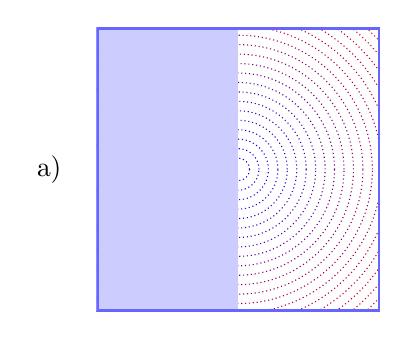
\begin{tikzpicture}[scale=1.2]
            \node[] at (-2, 0) {a)};
            \begin{scope}
                \clip (-1.5, -1.5) rectangle (1.5, 1.5);
                \foreach \cRadius in {1, ..., 22}
                    \pgfmathsetmacro\cColor{\cRadius/22*100}
                    \draw[red!\cColor!blue, densely dotted] (0, 0) circle (0.02+\cRadius*0.1); 
                    
                \fill[blue!20] (-1.5, -1.5) rectangle (0, 1.5);
                \draw[blue!60, ultra thick] (-1.5, -1.5) rectangle (1.5, 1.5);
            \end{scope}
        \end{tikzpicture}
        \qquad
        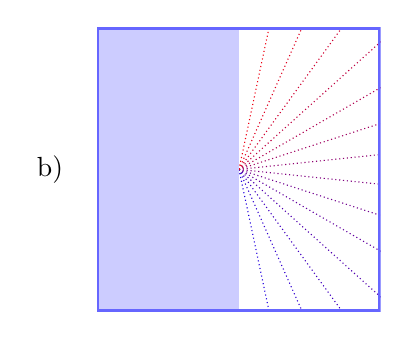
\begin{tikzpicture}[scale=1.2]
            \node[] at (-2, 0) {b)};
            \begin{scope}
                \clip (-1.5, -1.5) rectangle (1.5, 1.5);
                \foreach \cAngle in {1, ..., 16}
                    \pgfmathsetmacro\cColor{\cAngle/16*100}
                    \draw[red!\cColor!blue, densely dotted] (0, 0) -- (\cAngle* 180 / 15 -102:3); 
                \fill[blue!20] (-1.5, -1.5) rectangle (0, 1.5);
                \draw[blue!60, ultra thick] (-1.5, -1.5) rectangle (1.5, 1.5);
            \end{scope}
        \end{tikzpicture}
    \end{center}
    \caption{Schéma représentant l'extraction de caractéristiques à partir de l'espace de Fourier. En a), l'utilisation de cercle concentrique depuis l'origine, schématisé en pointillés; En b), l'extraction selon une direction.}
    \label{fig:scheme_fourier_features}
\end{figure}\par

La transformée en ondelettes possède divers avantages dont une bonne capacité de localisation, par translation de l'ondelette mère, et la possibilité de prendre en considération plusieurs échelles d'analyse, par homothétie~\cite{Livens1997,Wiltgen2008}. Concernant le choix de l'ondelette mère, celui-ci ne semble pas affecter la qualité des caractéristiques extraites~\cite{Fatemi1996, Livens1997}. Néanmoins, l'un des auteurs préconise le choix d'ondelette symétrique ou anti-symétrique~\cite{Livens1997}. Plusieurs de nos références s'orientant vers des ondelettes de Daubechies, nous privilégierons ces dernières~\cite{Wiltgen2008,Halimi2017a}. La décomposition est ainsi réalisée à divers niveaux afin de capter plusieurs niveaux de détail. La décomposition d'un niveau se réalise en 3 étapes successives: 
\begin{inlinerate}
    \item de filtrage passe-bas et passe-haut horizontal,
    \item de filtrage passe-bas et passe-haut vertical,
    \item puis une étape de sous-échantillonage afin de réduire limiter la quantité d'information.
\end{inlinerate} Les mesures statistiques extraites préconisés à ces diverse échelles sont la déviation standard, l'énergie et l'entropie~\cite{Livens1997, Wiltgen2008}. La transformée en ondelettes sera effectuée dans le reste de ce travail par la bibliothèque logicielle "PyWavelets" \cite{lee2006pywavelets}.\par

\begin{figure}[H]
\centering
    \begin{subfigure}{.45\textwidth}
      \centering
      \includegraphics[width=\linewidth]{contents/chapter_4/resources/scheme_dwt.pdf}
    \end{subfigure}
    \vrule
    \begin{subfigure}{.45\textwidth}
      \centering
      \includegraphics[width=\linewidth]{contents/chapter_4/resources/scheme_dwt_decomposition.pdf}
    \end{subfigure}
    \caption{Principe de la décomposition en ondelettes appliquée aux images~\cite{Livens1997}. A gauche, la décomposition est réalisée en trois temps. Un filtrage passe bas (L) et passe haut (H) sont réalisés selon la direction horizontale, puis selon la direction verticale. Enfin, un sous échantillonage de coefficient 2 est appliqué afin d'obtenir un matrice de même taille que l'image d'origine. A droite, les  deux principaux types de décomposition successives: par schéma pyramidal ou arbre dyadique, et par structure d'arbre.}
    \label{fig:photography_example}
\end{figure}\par

Le premier travail réalisé par Wiltgen~\cite{Wiltgen2008} met à disposition deux méthodes d'extraction de caractéristiques à partir de transformations fréquentielles desquelles sont obtenues diverses statistiques. Dans un premier temps, une de ses méthode se base sur la transformée de Fourier, et extrait \textbf{38 descripteurs} de la magnitude du spectre:
\begin{itemize}
    \item \textbf{22 descripteurs} correspondent à la moyenne calculée sur des rayons répartis de manière équidistante du centre du spectre (\label{fig:scheme_fourier_features} - a ),
    \item \textbf{16 descripteurs} correspondent à la moyenne calculée sur des directions à intervalles constantes (\label{fig:scheme_fourier_features} - b ).
\end{itemize} Dans un second temps, ce même article propose un approche par ondelettes de Daubechies. La transformée est ainsi calculée à cinq niveau successif sous forme d'arbre diadique, et préconise l'extraction de 3 mesures statistiques (la déviation standard, l'énergie et l'entropie) par bande de fréquences pour un total de \textbf{39 descripteurs}.\par

Le second travail sur lequel nous nous appuyons est une forme d'extension de la transformée en ondelettes du précédent travail~\cite{Halimi2017a}. Cette transformée est réalisée de manière diadique à quatre niveaux différents de décomposition. L'auteur y propose une extraction statistique différente des précédents travaux, reposant sur une approximation à chaque niveau de décomposition par une loi normale généralisée centrée dont la densité de probabilité $f$ est décrite par l'\Cref{eq:ggd}. Les auteurs de l'étude ne retiennent comme caractéristiques que les paramètres d'échelle $\alpha$ et de forme $\beta$.\par
\begin{equation}
    f(x)= \frac{\beta}{2\alpha\Gamma(1/\beta)} e^{-\left(|\frac{x}{\alpha}|\right)^\beta}
    \label{eq:ggd}
\end{equation}
 
Ainsi, nous réaliserons plusieurs expériences sur base de descripteurs manuels en fréquence. Dans un premier temps, nous tenterons d'étudier l'impact des méthodes standards. Puis dans un second temps, nous reproduirons les méthodes de la littérature proche de notre thématique et précédemment détaillés~\cite{Wiltgen2008, Halimi2017a}. La \Cref{tab:number_features_frequency} synthétise le nombre associé de caractéristiques extraites par ces diverses méthodes d'extraction fréquentielles.\par

\begin{table}[h]
\centering
    \begin{tabular*}{0.6\linewidth}{l@{\extracolsep{\fill}}l}
        \hline
        \textbf{Méthode}                        & \textbf{Nombre}   \\ \hline
        Fourier                                 & XX                \\ \hline
        Ondelettes                              & XX                \\ \hline
        Wiltgen~\cite{Wiltgen2008} - Fourier    & 38(22+16)         \\ \hline
        Wiltgen~\cite{Wiltgen2008} - Ondelettes & 39(13$\times$3)   \\ \hline
        Halimi~\cite{Halimi2017a} - Ondelettes  & 24(12$\times$2)   \\ \hline
    \end{tabular*}
    \caption{Nombre de caractéristiques extraites par méthode spatiale.}
    \label{tab:number_features_frequency}
\end{table}\par

\subsubsection{Technique d'apprentissage par transfert de connaissances}
Les techniques d'apprentissage par transfert de connaissances sont un champs d'application relativement récent en comparaison des techniques d'apprentissage automatique. Le principe est la réutilisation de connaissances précédemment acquises dans le but de résoudre de nouveau problèmes plus rapidement, voir plus efficacement. Pour cela, ce champs vise à  proposer des moyens d'extraire les connaissances d'une ou plusieurs tâches sources, et de les appliquer à une tâche cible~\cite{QiangYang2010}.\par

Les technique par transfert de connaissances sont assez récente dans la littérature est proviennent d'une émergence de la recherche sur les \gls{cnn}. Elles sont une réponse à de nombreuses problématiques autour de l'entraînement des \gls{cnn}: 
\begin{inlinerate}
    \item ses contraintes matérielles,
    \item ses contraintes de données,
    \item et la complexité liée à l'entraînement.
\end{inlinerate}
ImageNet\cite{Deng2008} why\cite{huh2016}
Nous utiliserons à cette fin une architecture de type "InceptionV3" supposée pertinente dans ce cadre d'application \cite{Litjens2017}. Afin de tirer le meilleur parti de cette architecture, nous nous orientons vers de l'apprentissage par transfert. En effet, ce type de techniques est particulièrement adapté à des problématiques suffisamment proche des données initiales, et pour lesquelles la quantité de données disponible est restreinte. Pour cela, nous nous référons à une version de ce modèle entraînée sur la base d'images "ImageNet", dont nous retirons au préalable les couches responsables de la classification. Afin de conserver une cohérence entre le nombre de caractéristiques extraites et le nombre d'échantillons à notre disposition, nous ajoutons également une couche de "Global Pooling" pour réduire la dimension spatiale de chaque carte d'activation à un simple scalaire. Lors de ces prochaines lignes, nous utilisons le terme "\ac{rnc} Max" (respectivement "\ac{rnc} Moy") pour faire référence à un tel réseau comportant respectivement une couche de "Global Pooling" basé sur une fonction de maximum (respectivement moyenne). De plus, nous combinons aux précédents éléments une \ac{pca} afin de réduire considérablement le nombre de variables de manière non supervisée et analyser son incidence. La manipulation des \ac{rnc} est réalisée grâce à la bibliothèque logicielle "Keras" \cite{chollet2015keras}.\par

The third category of methods investigated was in regard to deep learning methods and more specifically in regard to \ac{cnn}, which are known to be well-suited methods for image classification, thanks to robust feature patterns~\cite{Pathan2018}. Many architectures were used to address ImageNet challenges, and their associated performances were analyzed~\cite{Canziani2016}. Instead of training this network from scratch, as we have data constraints and also computational constraints, we choose a Domain Adaptation approach for these models. Most of the papers to date have dealt with \ac{cnn} trained on ImageNet~\cite{Deng2008}, as this database contains thousands of classes and more than 14 million images, meaning that the extracted features from these networks can be used in various fields. As discussed in a previous work~\cite{Litjens2017}, Inception-V3 architecture pre-trained on ImageNet is thought to be the most relevant for medical applications. As \ac{rcm} images can have various forms and can contain specifics details compared to other image modalities, this research compares the most well known \ac{cnn} architectures: VGG-16~\cite{Simonyan2014}, Inception-V3~\cite{Szegedy2015}, ResNet~\cite{He2016} and Inception-ResNet~\cite{Szegedy2017}, with accuracies of 0.71, 0.76, 0.78, and 0.80, respectively, on the ImageNet database~\cite{Canziani2016}. This method involves the use of Transfer Learning, by removing the last layers devoted to the classification task, in order to obtain a new representation of the image data as features. Furthermore, in order to reduce the number of features provided by the previous step, a global pooling layer on each activation layer was performed.
L'ensemble des réseaux employés et paramètres extraits associés sont résumés au sein de la \Cref{tab:number_features_transferlearning}.\par

\begin{table}[H]
    \centering
    \begin{tabular*}{0.6\linewidth}{l@{\extracolsep{\fill}}l}
    \hline
    \textbf{Architecture}        & \textbf{Nombre}          \\ \hline
    VGG-16                       & 512                      \\ \hline
    Inception-V3                 & 2048                     \\ \hline
    ResNet                       & 2048                     \\ \hline 
    Inception-ResNet             & 1536                     \\ \hline
    \end{tabular*}
    \caption{Nombre de caractéristiques extraites par type d'architecture de \gls{rnc}.}
    \label{tab:number_features_transferlearning}
\end{table}\par

\subsubsection{Pré analyse}
\begin{figure}[H]
    \centering
    \includegraphics[width=\linewidth]{contents/chapter_4/resources/example_glcm.pdf}
    \caption{Exemple d'extraction de \gls{glcm} de second ordre sur deux images typique. En haut, un cas d'image bénigne; En bas, une image pathologique typique de \gls{lm}.}
    \label{fig:example_glcm}
\end{figure}\par

\begin{figure}[H]
    \centering
    \includegraphics[width=\linewidth]{contents/chapter_4/resources/example_fft.pdf}
    \caption{Exemple de transformée de Fourier appliquée à deux images typiques, représentation selon le module et la phase. En haut, un cas d'image bénigne; En bas, une image pathologique typique de \gls{lm}.}
    \label{fig:example_fft}
\end{figure}\par

\begin{figure}[H]
    \centering
    \includegraphics[width=\linewidth]{contents/chapter_4/resources/example_wavelet.pdf}
    \caption{Exemple de transformée en ondelettes (Daubechies) appliquée à deux images typiques, à 2, 3 puis 4 niveaux. En haut, un cas d'image bénigne; En bas, une image pathologique typique de \gls{lm}.}
    \label{fig:example_wavelet}
\end{figure}\par

\subsection{Balancement de données}
\subsection{Post Traitements}
\subsubsection{Normalisation}
\subsubsection{Réduction de l'information}
dct/pca~\cite{Nanni2017}
\subsection{Méthodes de prédiction}
\section{Processus d'apprentissage profond convolutionnel}
\subsection{Augmentation de données}
\subsection{Programme d'apprentissage}
\subsection{Fonction de coût}
\subsection{Réglages fin}
\section{Résultats}

% \label{sec:features}
% In order to classify the data, a reduction of the image information had to be performed in a new feature space able to distinguish “malignant” from “benign” image types. According to the dermatologists, texture plays an important role in the differentiation of tissue types. The first part of this section focuses on handcrafted feature extractors based on texture from previous work~\cite{Wiltgen2008}. The deep extraction methods applied to this context and inspired by a previous work on dermoscopy images~\cite{Esteva2017} are then detailed. All of the feature extraction methods are listed in \Cref{tab:features_methods}, and the next parts follow this table structure.\par
% \begin{table}[H]
%     \centering
%     \begin{tabular}{lll}
%     \hline
%     \textbf{Category}                   &  \textbf{Name}                & \textbf{Number of features}  \\ \hline
%     \multirow{2}{*}{Spatial}            &  Haralick                     & 12                        \\ \cline{2-3} 
%                                         &  \gls{glh}+\gls{glcm}         & 17                        \\ \hline 
%     \multirow{2}{*}{Frequency}          &  Fourier                      & 38                        \\ \cline{2-3} 
%                                         &  Wavelet                      & 39                        \\ \hline
%     \multirow{4}{*}{Transfer Learning}  &  VGG-16                       & 512                       \\ \cline{2-3} 
%                                         &  Inception-V3                 & 2048                      \\ \cline{2-3} 
%                                         &  ResNet                       & 2048                      \\ \cline{2-3} 
%                                         &  Inception-ResNet             & 1536                      \\ \hline
%     \end{tabular}
%     \caption{The list of all of the feature extraction methods performed in this paper and their associated extracted number of features.}
%     \label{tab:features_methods}
% \end{table}\par
% The “Spatial” extraction methods were based on spatial patterns of pixels, by use of \ac{glh} and \ac{glcm}. The method called “Haralick” refers to previous work based on texture features~\cite{Haralick1973} and it uses the \ac{glcm} concept by computation of the twelve statistical characteristics listed in \Cref{tab:histogram_features} - \ac{glcm} Features column. These characteristics were extracted along horizontal, vertical, and two diagonals. A mean was computed along these axes as the tissues are not oriented in space, and to reduce the number of features. A second method from previous work~\cite{Wiltgen2008}, called “\ac{glh}+\ac{glcm}” in this paper, expanded the first twelve initial characteristics of Haralick and it added five others based on \ac{glh}. In total, 17 features were extracted for each image, and all of the statistical properties extracted are listed in \Cref{tab:histogram_features}. The Haralick features extraction was performed using the “Mahotas” library~\cite{coelho2012mahotas} and histogram feature extraction was computed with help from the “Scipy” library~\cite{Jones2001}.\par
% \begin{table}[H]
%     \centering
%     \begin{tabular}{ll}
%         \hline
%         \textbf{\ac{glcm} Features}& \textbf{\ac{glh} Features}     \\ \hline
%         Angular Second Moment      & Mean value                     \\
%         Difference Moment          & Mean square deviation          \\
%         Correlation                & Skewness                       \\
%         Sum of Squares             & Kurtosis                       \\
%         Inverse Difference Moment  & Entropy                        \\     
%         Summed Average             &                                \\    
%         Sum Variance               &                                \\    
%         Entropy                    &                                \\    
%         Sum Entropy                &                                \\    
%         Difference Entropy         &                                \\    
%         Measure of Correlation 1   &                                \\  
%         Measure of Correlation 2   &                                \\ 
%     \end{tabular}
%     \caption{The statistical measures derived from \ac{glcm} and \ac{glh}, respectively, and extracted in order to perform “Spatial” extraction methods.}
%     \label{tab:histogram_features}
% \end{table}\par
% The second category of extraction methods, called “Frequency”, refers to a set of methods based on frequency approaches. The first method of this category is called “Fourier” and is based on the Fourier transform. The main idea is to provide different levels of information as high frequency refers to high-contrast parts and low frequencies to homogeneous areas in the image. As the spectrum is symmetrical around the origin, only half of this spectrum was considered for the sake of computational efficiency. Then, a mean value was computed for all of the coefficients located at the same radial distance from the origin, at 22 different radius sizes between 0 and the diagonal size of the image. A previous paper~\cite{Smach2008a} has also shown the relevance of this method in the context of textural images. Finally, 16 constant directions were taken from the origin of the power spectrum, and a mean value was computed for each of them~\cite{Wiltgen2008}. The second method of this category is called “Wavelet” in this work and is based on Wavelet transform by use of a decomposition based on a Daubechies 4 that provides quite fine localization properties~\cite{Wiltgen2008}. This decomposition was made at five scales, and only the four last scales were considered to compute coefficients. For each of them, three statistical measures were computed: the standard deviation, the energy, and the entropy.\par
% The third category of methods investigated was in regard to deep learning methods and more specifically in regard to \ac{cnn}, which are known to be well-suited methods for image classification, thanks to robust feature patterns~\cite{Pathan2018}. Many architectures were used to address ImageNet challenges, and their associated performances were analyzed~\cite{Canziani2016}. Instead of training this network from scratch, as we have data constraints and also computational constraints, we choose a Domain Adaptation approach for these models. Most of the papers to date have dealt with \ac{cnn} trained on ImageNet~\cite{Deng2008}, as this database contains thousands of classes and more than 14 million images, meaning that the extracted features from these networks can be used in various fields. As discussed in a previous work~\cite{Litjens2017}, Inception-V3 architecture pre-trained on ImageNet is thought to be the most relevant for medical applications. As \ac{rcm} images can have various forms and can contain specifics details compared to other image modalities, this research compares the most well known \ac{cnn} architectures: VGG-16~\cite{Simonyan2014}, Inception-V3~\cite{Szegedy2015}, ResNet~\cite{He2016} and Inception-ResNet~\cite{Szegedy2017}, with accuracies of 0.71, 0.76, 0.78, and 0.80, respectively, on the ImageNet database~\cite{Canziani2016}. This method involves the use of Transfer Learning, by removing the last layers devoted to the classification task, in order to obtain a new representation of the image data as features. Furthermore, in order to reduce the number of features provided by the previous step, a global pooling layer on each activation layer was performed. For convenience, this whole method is called “Transfer Learning” in the next paragraphs and the names of the respective networks are used. The \ac{cnn} computation was implemented using the “Keras” library~\cite{chollet2015keras}.\par

% %=====================================
% % IMAGE LEVEL
% %=====================================
% \subsection{Image-level decision}
% \label{sec:image_decision}
% The image-level decision was the first level of classification achieved in this study, whereby the image classification must be carried out according to the two classes “malignant”, as the positive class, and “benign”. In order to satisfy this objective, the process consisted of using the image as a single instance that has several discriminant characteristics and sufficient information to allow its classification. As formulated by~\cite{foulds_frank_2010}, such a problem can be set as a pair {X|y}, in which \(X=\{x_1,x_2,\ldots,x_n\}\) is a vector characteristic for which \(n\) is the number of features and \(y\) the associated label. The task consisted of finding the existing relationship between \(X\) and \(y\), using a classification process.\par 
% \begin{figure}[H]
%     \begin{center}
%         \includegraphics[width=0.7\linewidth]{Figures/Process_Image.pdf}
%         \caption{The classification process performed on the \ac{rcm} images. The “Extraction” box refers to one of the Feature Extraction methods mentioned in \Cref{sec:features}. The “Fit Model” and “Prediction” boxes are related to the training and inference steps, respectively, of one of the trained and inferred models discussed in \Cref{sec:image_decision}. The testing set was predicted based on two classes: “benign” and “malignant”}
%         \label{fig:image_process}
%     \end{center} 
% \end{figure}\par
% To achieve this task, an extraction method (see \Cref{sec:features}) was applied to the images, depending on the currently evaluated method. The features were then normalized based on a standard score computation to make the classification task more accurate and robust~\cite{Graf2001}. This scaling was computed by subtracting the mean and then dividing by the standard deviation. The schematic outline in \Cref{fig:image_process} provides an overview of this process.\par
% \begin{table}[H]
%     \centering
%     \begin{tabular}{lll}
%     \textbf{Name}                                   & \textbf{Parameter}& \textbf{Values}                           \\ \hline
%     \multirow{2}{*}{\ac{cart}/\acs{rf}/\acs{ert}}   & Maximum depth     & [3, $\infty$]                             \\ \cline{2-3}
%     \acreset{rf}\acreset{ert}                       & Criterion         & [Gini, Entropy]                           \\ \hline 
%     \multirow{2}{*}{\acs{gb}}                       & Maximum depth     & [3, $\infty$]                             \\ \cline{2-3}
%     \acreset{gb}                                    & Criterion         & [Mean squared error, Mean absolute error] \\ \hline 
%     \acs{svm} - Linear                              & C                 & [0.01, 0.1, 1, 10, 100, 1000]             \\ \hline
%     \multirow{2}{*}{\acs{svm} - RBF}                & C                 & [0.01, 0.1, 1, 10, 100, 1000]             \\ \cline{2-3}
%     \acreset{svm}                                   & Gamma             & [0.01, 0.1, 1, 10, 100, 1000]             \\ \hline 
%     \end{tabular}    
%     \caption{List of all of the classification models performed in this study and their referring evaluated hyper-parameters.}
%     \label{tab:image_hyperparameters}
% \end{table}\par
% Finally, the classification was performed on scaled features using different models. In the first stage, \ac{cart} was investigated as in a previous study in the same data context~\cite{Wiltgen2008}. In a second stage, this study explored alternatives of simple trees based on ensemble methods (set of models instead of a single model) as the \ac{cart} model tends to overfit. On the one hand, bagging methods were investigated by the use of \ac{rf} model~\cite{Breiman2001} and \ac{ert}~\cite{Geurts2006} as they both tend to remove the overfitting issues. Moreover, the \ac{ert} model are assumed to be more robust to noise than the \ac{rf} model. On the other hand, the boosting method was considered by the use of the \ac{gb} model~\cite{Friedman2000} as the most common type of tree-based algorithm for most of the recent applications. Lastly, \ac{svm} models were evaluated that are known to be suitable in multiples contexts~\cite{Smach2008a,Kose2016b}. As the relationship between the features and the expected outputs can be complex, \ac{svm} models were compared over linear and RBF kernels.\par
% In addition, to provide the best performance with each of these models, a search in regard to their optimum hyperparameters was carried out (see \Cref{tab:image_hyperparameters}).\par

% The validation protocol remains the same for each of these experiments, based on a nested cross-validation that is known to be less biased than a simple cross-validation scheme~\cite{Cawley2010}. This protocol allows 1) cross-validation of hyper-parameters and 2) objective evaluation of the prediction models. Each of the cross-validation step is based on a K-fold strategy with a $k$ value of 4 on the testing loop and 2 on the validation loop. Also, each time, the patients are separated and balanced as best as possible based on the image labels. In order to achieve an objective evaluation, each data cluster remains the same for the experiments in a given section (refer to \Cref{sec:image_decision} and \Cref{sec:patient_decision}). Moreover, each experiment is validated and evaluated using a \fscore{} metric, as it is statistically suitable for unbalanced populations in comparison with accuracy, and it represents in a single value both recall and precision information. In addition, standard deviation is computed to analyse the stability of models along the nested cross-validation. For this purpose, we used the “Scikit Learn” library for Machine Learning classification, validation, and metric~\cite{pedregosa2011scikit}.\par

% The results of \Cref{sec:image_decision} regarding image-level decisions were performed only on the labeled images and are listed in \Cref{tab:image_results}. The most suitable handcrafted extraction method was based on the “Wavelet” method combined with the “\ac{svm} - Linear” model, reaching an weighted \fscore{} of 0.74 with stable performance of 0.04. In general, all of the handcrafted methods performed in a quite similar and stable way, varying from 0.69 to 0.74 for the \fscore{} and 0.03 to 0.07 for the deviation. In addition, the Transfer Learning-based feature extraction reached higher scores with the “\ac{svm} - Linear” model, in particular with the “Inception-ResNet” architecture, which achieved a weighted \fscore{} of 0.82 with a deviation of 0.04. With this same model, the Transfer Learning feature extraction methods varied from 0.76 to 0.82, with a deviation range from 0.02 to 0.04. By contrast, all of these architectures were poorly processed by the “\ac{svm} - RBF” model and can be explained by the high-dimensionality of the extracted features that resulted in overfitting despite the cross-validation of the regularization term. In this situation, the “VGG-16” architecture was more suitable with only 512 features than the remaining architectures providing 1,536 or 2,048 features. In regards to tree-based models, the \ac{cart} model weighted \fscore{} varies between 0.69 and 0.71 (deviation between 0.03 and 0.05) and 0.58 to 0.64 (deviation between 0.02 and 0.12), respectively for handcrafted methods and transfer learning methods. On the other hand, the \ac{gb} model weighted \fscore{} varies from 0.67 to 0.73 (deviation between 0.04 and 0.07) and 0.78 to 0.81 (deviation between 0.04 and 0.05). The above two sentences can be explained by an overfit in a high dimensional situation for the \ac{cart} model and in a low dimensional situation for the \ac{gb} model. In opposition, the \ac{rf} and \ac{ert} models were homogeneous along with handcrafted and transfer learning features as they are less prone to overfitting in both low and high dimensional feature spaces. To sum up the aforementioned results, the rest of this article retains only the best combination, with “Inception-ResNet” as the feature extraction methods and the Linear \ac{svm} as the classification model.\par



Néanmoins, il est également a été également jugées important de l'intersection d'évènements tels que la présence de tissus caractéristiques aux abords de follicules pileux.\par